\documentclass[11pt,a4paper]{ivoa}
\input tthdefs

\newcommand{\xtype}[1]{\texttt{#1}}
\newcommand{\ucd}[1]{\texttt{#1}}

\usepackage{listings}
\lstloadlanguages{XML,sh}
\lstset{flexiblecolumns=true,basicstyle=\small,tagstyle=\ttfamily}
\usepackage[utf8]{inputenc}
\usepackage{todonotes}
\usepackage{textcomp}
\usepackage{float}
\usepackage{lscape}
\usepackage{longtable}

\title{IVOA Obscore Extension for Visibility data}

\ivoagroup{Data Model Working Group}

\author{Fran\c cois Bonnarel}
\author{Mireille Louys}
\author{Mark Kettenis}
\author{Mark Lacy}
\author{Mattia Mancini}


\editor{Fran\c cois Bonnarel}

\previousversion{}

       


\begin{document}

\begin{abstract}
	This is a proposed extension to the Obscore specification for description of visibility data
\end{abstract}

\section*{Acknowledgments}

The authors would like to thank all the participants in DM-WG and Radioastronomy-IG discussions  for their ideas, critical reviews, and contributions to this document.

\section{Introduction}
ObsCore specification \citep{std:OBSCORE} defines both a minimal datamodel to describe datasets and a table consistent with the model which can be served by Tap services. It has been successful to define a lot of data discovery services in astronomy.

The emergence of the Radioastronomy interest group in the IVOA in April 2020 showed the strong interest of the radio astronomy community to distribute their data in the VO. A lot of groups now distribute their data using VO standards\footnote{https://ivoa.net/documents/Notes/RadioVOImp/index.html} If reduced spectral cubes (and single dish data - {\it is that true ?} ) fit well with ObsCore, the situation is a bit different for interferometry visibility data. This was already exposedin 2010 when Anita Richards wrote a note called "Radio interferometry data in the VO"\footnote{https://wiki.ivoa.net/internal/IVOA/SiaInterface/Anita-InterferometryVO.pdf} which is still worth reading. The current specification tries to find solutions for that. 
 
Although the interferometry data are nowadays dominent in radio field, similar issues occur for optical interferometry data. The extension we are defining here is valid for both domains.  


\begin{figure}[H]
\centering

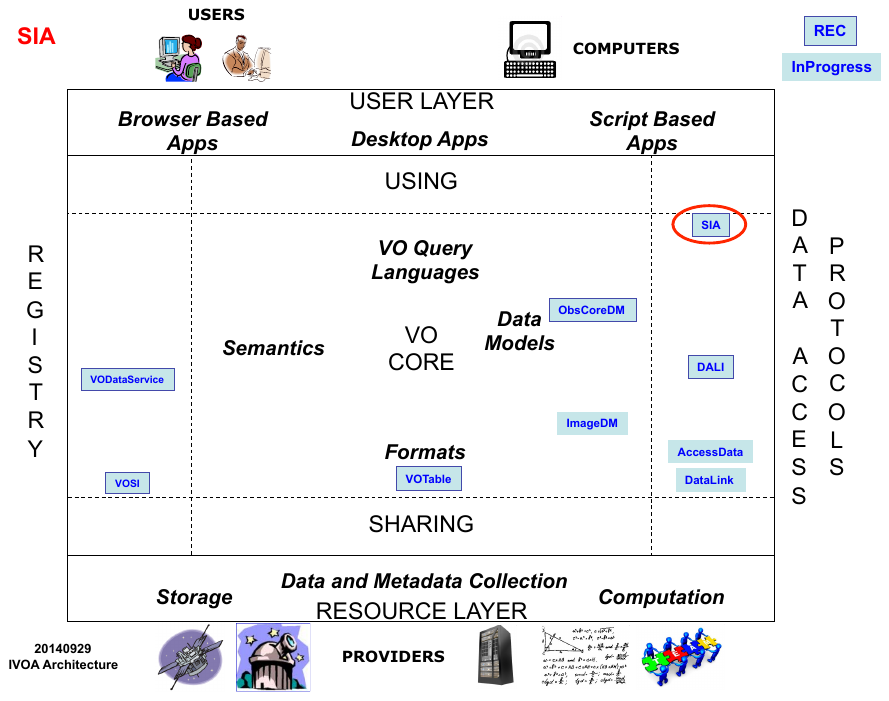
\includegraphics[width=0.9\textwidth]{archdiag.png}
\label{fig:architecture}
\end{figure}


The role of this Visibility ObsCore extension in the IVOA is very close to ObsCore itself. It's only a fine grain improvement of this specification. 



\section{Visibility data specificities from the Data discovery point of view}
\label{sec:specificities}

    Visibility data are sets of  complex number measurements giving amplitude and phase of interference franges obtained for a given field in sky, a given time, a given wavelength or polarisation. 

    They can be organized in the following way : catalogs of matrices of measurements for various fields and settings of the antennae pairs distances and orientation. Matrices are regulary sampled in time, wavelength and polarisation.
    
    On the other side they are sparsed in the spatial fourier transform space (also called the uv plane) because it's impossible to cover regularly this space with a limited number of antennae pairs.
    

    How can the Obscore parameters describe the characterization of these observations ?
    Obviously if there are several "fields" in the observation, these different fields would have to be described in several records of the Obscore table because the s\_ra and s\_dec parameters have to be unique.

   Spectral and Time axis are regularly sampled but we can have gaps between time and spectral intervals. In addition, on the spectral axis different samplings may coexist.  
   
   
    Again a visibility observation will be splitted in several ObsCore records in order to ensure the consistency of the time and spectral characterization parameters of each unit.
    

    Finally, visibility measurements can be either integrated for all polarisations or splitted in the different polarisation parameters (Stokes or whatever) 

    
    We consider that  consistent ObsCore records as described above defines  "visibility" datasets in the sense of ObsCore.

    Radio Astronomers generally make use of frequencies for designating the spectral ranges of their observation. The standard ObsCore attributes em\_min em\_max  are in wavelength  andare not really convenient for them. That's why wde should also provide  their translation into frequencies. 
        
    Moreover visibility data show some dependency of the spatial field of view and resolution with wavelength. Generally only a typical value for these two numbers can be given. 
    Contrary to what occurs with direct spatial observations, large scales may also be filtered as are small scales This depends of the smallest distance in the frequency plane.
    For large spectral ranges, the variations of fov and resolution along the axis may become so large that the typical value cannot be sufficient to characterize the dataset. 
    Ranges of values for fov size and resolution will achieve this task more accurately

     The quality of the data strongly depends from the distribution of the visibility measurements in the uv plane : the more complete will be the sampling, the better will be the recosntructed image. The uv plane distribution can be characterized by several numbers.The minimal and maximum distance between measurements in the uv plane are important to get the actual resolution and largest angular scale. Beside this a uv plane filling factor of the distribution  will allow to predict the quality of reconstruction.
          Eventually, the ellipticity of the distribution is a measure of the distortions that can affect the reconstruction.
          
          Radioastronomers also check the quality of the visibility data by looking at some maps  of the data structure.           The Uv coverage map can show how complete and regular is the sampling in the uv plane and give an hint of resolution and maximum angular scale
The visualisation of the dirty beam, which is the fourier transform of the uv sampling function gives an hint of the intrinsec quality of possible reconstruction./As maps they are not queriable. So it is questionable if links to this maps are to be exposed in the extension table or only via a DataLink service. 
          
          If none of these uv characterization features are available to be exposed in the service we can stil predict ranges of some of those by using some kind of facility description.  
          Important features are the antenna diameter (or maximum antenna parameter) the number of antennane and the minimum and maximum distance between antennane of the array.
          
           



\section{ObsCore attributes definition valid for visibility data}
\label{sec:ObsCoreVisDef}

Some mandatory or optional parameters will have peculiar estimation for visibility data.

\subsection{obs\_id}

Astronomers usually know what they identify as a single observation : a complex set of measurements made in given sequence of time. obs\_id should define unambiguously each observation.

\subsection{obs\_publisher\_did}

Visibility data observations are generally splitted in several subparts with consistent characterozation parameters described by a single ObsCore record. Each of these records is consiedered as describing a dataset and has its own obs\_publisher\_did. It has to be unique in the virtual observatory.

\subsection{s\_fov}
\label{sec:fov}

A typical value for the field of view size will be given by $\lambda / D$ where $\lambda$ is the mid value of the spectral range and D is the largest diameter of the array antennae or telescopes.
 
\subsection{s\_resolution}
\label{sec:res}

A typical value for the spatial resolution will be given by $\lambda / L$ where $\lambda$ is the mid value of the spectral range and L is the longest distance in the uv plane. 

\subsection{s\_region}

This shape will be the typical contour of the detectable beam. Of course it cannot be accurate. 

\subsection{o\_ucd}

In the case of visibility data the "observable" is a complex number representing fourier coefficients of the image Fourier transform. Its ucd is stat.fourier. 

\subsection{t\_exptime}

\subsection{t\_resolution}


\section{ObsCore extension for visibility data}

Table \ref{tab:ExtensionAtt} shows the additional parameters we propose to add to ObsCore in order to better describe visibility data.
In TAP or SIA services, they can be added to the main ObsCore table or provided in an extra table which will be joined to the main table. 
\subsection{spatial parameters}

The s\_maximum\_angular\_scale is estimated as $\lambda/l$ where $\lambda$ is the typical wavelength and l is the smallest distance in the uv plane. s\_fov\_min, s\_fov\_max, s\_resolution\_min, s\_resolution\_max are estimated like the typical values (see subsections \ref{sec:fov} and \ref{sec:res} ) where $\lambda$ is replaced by the minimum and maximum wavelength of the spectral ranges

\subsection{time parameters}

t\_exp\_min and t\_exp\_max are added because of strong variation in the individual time stamps duration.

\subsection{uv parameters}
uv\_distance\_min and uv\_distance\_max are straigthforward.
To compute the eccentricity of the UV distribution a principal component analysis (PCA) with 2 components is performed over the data points sampling the UV plane to select the main axis of data scattering. The first component is used to rotate the distribution of UV in a way that the major variation of the distribution is leaning towards the $x$ axis of a bi dimensional $xy$ Cartesian plane. The major axis length and the minor axis length of the ellipse are therefore defined as the semi distance between the most positive point along the $x$/$y$ axis and the most negative point among the $x/y$ axis. For instance, if the range of the rotated UV will cover on the $x \in [-10, 10]$ the major axis distance would be 10, a similar procedure is done on the y axis. This procedure allow the definition of the UV distribution eccentricity (
uv\_distribution\_exc) computed as follows:
\begin{equation}
uv\_distribution\_exc = \sqrt{1-\frac{b^2}{a^2}}
\end{equation}
where a is the major axis length and b is the minor axis length.
The filling factor of the UV plane (hereafter uv\_distribution\_fill) is computed as the average number of samples found in a $N^{uv}_{samples}$x$N^{uv}_{samples}$ equispaced grid enclosing the rotated ellipse. In formulas,
 the boundaries of a cell (i,j) are defined by the boundaries
\begin{equation}
u \in [u_{min} + \frac{u_{max} - u_{min}}{N^{uv}_{samples}} \cdot i , u_{min} + \frac{u_{max} - u_{min}}{N^{uv}_{samples}} \cdot (i + 1)]
\end{equation} 
and
\begin{equation}
v \in [v_{min} + \frac{v_{max} - v_{min}}{N^{uv}_{samples}} \cdot j , v_{min} + \frac{v_{max} - v_{min}}{N^{uv}_{samples}} \cdot (j + 1)]
\end{equation} 
where $u_{max}$/$v_{max}$ are the respective maximum u/v of the uv sample and $u_{min}$/$v_{min}$ is the minimum u/v of the uv sample.

Given the above boundaries the number of samples within a cell (i,j) will be $n^{uv}_{i,j}$ and uv\_distribution\_fill will be then computed as 
\begin{equation}
uv\_distribution\_fill = \frac{\sum^{N^{uv}_{samples}}_{i=1} \sum^{N^{uv}_{samples}}_{j=1} n^{uv}_{i,j} }{(N^{uv}_{samples}) ^ 2},
\end{equation}

in the preliminary analysis $N^{uv}_{samples} = 1000$.

\subsection{instrumental parameters}

They all give a predefined raw idea of resolution, field of view, maximum angular scale and sampling quality.

\subsection{uv coverage and dirty beam map}

These uv\_coverage\_map and s\_resolution\_beam\_dirty parameters are  intended to be url to files containing these maps. 
Implementers may want to avoid adding url columns to the ObsCore table. In that case DataLink \citep{std:DataLink} may provide a solution. The semantics FIELD in the \{link\} response    will contain \#auxiliary  for links to this map while  the content\_qualifier FIELD could contain the utype.

        
\begin{landscape}
\begin{longtable}{l  p{4cm} p{4cm} p{4cm} l l}
\sptablerule
\textbf{column name}&\textbf{definition}&\textbf{utype}&\textbf{ucd}&\textbf{unit}\cr
\sptablerule
\sptablerule
\texttt{ s\_resolution\_min}&\texttt{ Angular resolution, longest baseline and  max frequency dependant}&{ Char.SpatialAxis.\newline Resolution.Bounds.\newline Limits.LoLim}&{pos.AngResol;stat.min}&{arcsec}\cr
\sptablerule
\texttt{s\_resolution\_max}&\texttt{Angular resolution, longest baseline and min frequency dependant}&\texttt{Char.SpatialAxis.\newline Resolution.Bounds.\newline Limits.HiLim}&{pos.AngResol;stat.max}&arcsec\cr
\sptablerule
\texttt{s\_fov\_min}&\texttt{field of view diameter,  min value, max frequency dependant}&\texttt{Char.SpatialAxis.\newline Coverage.Bounds.\newline Extent.LowLim}&{phys.angSize;instr.fov;\newline stat.min}&deg\cr
\sptablerule
\texttt{s\_fov\_max}&\texttt{field of view diameter,  max value, min frequency dependant}&\texttt{Char.SpatialAxis.\newline Coverage.Bounds.\newline Extent.HiLim}&{phys.angSize;instr.fov;\newline stat.max}&deg\cr
\sptablerule
\texttt{s\_maximum\_angular\_scale}&\texttt{maximum scale in dataset, shortest baseline and  frequency dependant}&\texttt{Char.SpatialAxis.\newline Resolution.Scale.\newline Limits.HiLim}&{phys.angSize;stat.max}&arcsec\cr
\sptablerule
\texttt{f\_min}&\texttt{spectral coverage min in frequency}&\texttt{Char.SpectralAxis.\newline Coverage.Bounds\newline Limits.LoLim}&{em.freq;stat.min}&Mhz\cr
\sptablerule
\texttt{f\_max}&\texttt{spectral coverage max in frequency}&\texttt{Char.SpectralAxis.\newline Coverage.Bounds\newline Limits.HiLim}&{em.freq;stat.max}&Mhz\cr
\texttt{t\_exp\_min}&\texttt{minimum integration time per sample}&\texttt{Char.TimeAxis.\newline Sampling.Extent\newline LoLim}&{time.duration;obs.exposure;\newline stat.min}&s\cr
\sptablerule
\texttt{t\_exp\_max}&\texttt{maximum integration time per sample}&\texttt{Char.TimeAxis.\newline Sampling.Extent\newline HiLim}&{time.duration;obs.exposure;\newline stat.max}&s\cr
\sptablerule
\texttt{uv\_distance\_min}&\texttt{minimal distance in uv plane}&\texttt{Char.UVAxis.\newline  Coverage.Bounds.\newline Limits.LoLim}&stat.fourier;pos;stat.min&m& \cr
\sptablerule
\texttt{uv\_distance\_max}&\texttt{maximal distance in uv plane}&\texttt{Char.UVAxis.\newline  Coverage.Bounds.\newline Limits.LoLim}&stat.fourier;pos;stat.max&m \cr
\sptablerule
\texttt{uv\_distribution\_exc}&\texttt{excentricity of uv distribution}&\texttt{Char.UVAxis.\newline  Coverage.Bounds.\newline Excentricity}&stat.fourier;pos& \cr
\sptablerule
\texttt{uv\_distribution\_fill}&\texttt{filling factor of uv distribution}&\texttt{Char.UVAxis.\newline  Coverage.Bounds.\newline FillingFactor}&stat.fourier;pos& \cr
\sptablerule
\texttt{instrument\_ant\_number}&\texttt{number of antennae in array}&\texttt{Provenance.ObsConfig.\newline Instrument.Array.\newline AntNumber}&instr.baseline;meta.number& \cr
\sptablerule
\texttt{instrument\_ant\_min\_dist}&\texttt{minimum distance between antennae in array}&\texttt{Provenance.ObsConfig.\newline Instrument.Array.\newline MinDist}&instr.baseline;stat.min&m \cr
\sptablerule
\texttt{instrument\_ant\_max\_dist}&\texttt{maximum distance between antennae in array}&\texttt{Provenance.ObsConfig.\newline Instrument.Array.\newline MaxDist}&instr.baseline;stat.max&m \cr
\sptablerule
\texttt{instrument\_ant\_diameter}&\texttt{diameter of antennae in array}&\texttt{Provenance.ObsConfig.\newline Instrument.Array.\newline Diameter}&instr&m \cr
\sptablerule
\texttt{uv\_distribution\_map}&\texttt{uv distribution map}&\texttt{Char.UVAxis.\newline  Sampling.\newline Sensitivity.Map}&stat.fourier;pos& \cr
\sptablerule
\texttt{s\_resolution\_beam\_dirty}&\texttt{dirty beam}&\texttt{Char.SpatialAxis.\newline Resolution.\newline Variability.DirtyBeam.\newline Map}&{pos.AngResol}&\cr

\caption{ObsCore visibility data extension parameters}
\label{tab:ExtensionAtt}
\end{longtable}
\end{landscape}


\bibliography{ivoatex/ivoabib}

\end{document}
